\documentclass[a4paper,11pt]{article}
\usepackage[utf8]{inputenc}\usepackage[T1]{fontenc}
\usepackage[english]{babel}\usepackage{lmodern}\usepackage{microtype}
\usepackage{amsmath,amssymb}\usepackage{geometry}
\geometry{a4paper,left=2.2cm,right=2.2cm,top=2.0cm,bottom=2.0cm}
\usepackage{booktabs,array}\usepackage{xcolor}
\definecolor{bokug}{RGB}{0,135,60}\usepackage{tikz}
\usetikzlibrary{arrows.meta,calc}
\usepackage{fancyhdr}\pagestyle{fancy}
\renewcommand{\headrulewidth}{0.4pt}
\usepackage{enumitem}\setlength{\parindent}{0pt}\setlength{\parskip}{4pt}

\begin{document}
\fancyhead[L]{\small VU Mechanik – LAWI 100515 (PI)}\fancyhead[R]{\small SS 2026}\fancyfoot[C]{\thepage}
\begin{center}{\large\bfseries\color{bokug}University of Natural Resources and Life Sciences, Vienna (BOKU)}\\[2pt]{\large\bfseries VU Mechanik – LAWI 100515 (PI)}\\[4pt]Exam \textbf{Group A} \hfill Date: 26.06.2026\\[2pt]\rule{\linewidth}{0.4pt}\end{center}

\begin{center}\textbf{\large Model solution}\end{center}
\begin{center}
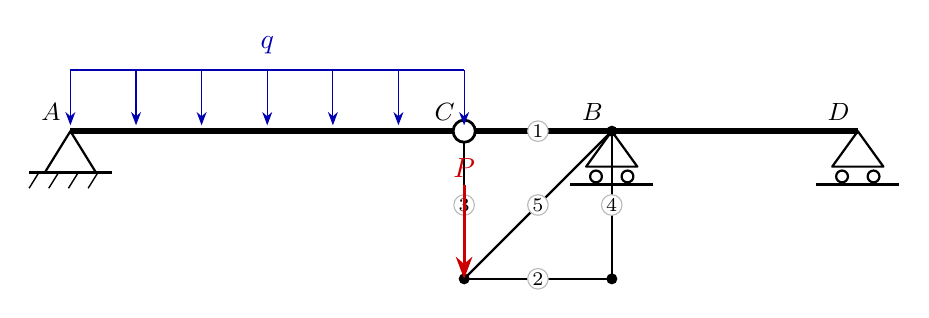
\begin{tikzpicture}[scale=1.250,>=Stealth,line join=round]
  \coordinate (P0) at (0.000,0.000);
  \coordinate (P1) at (4.000,0.000);
  \coordinate (P2) at (8.000,0.000);
  \coordinate (TO1) at (5.500,0.000);
  \coordinate (TU0) at (4.000,-1.500);
  \coordinate (TU1) at (5.500,-1.500);
  \draw[thick] (P1) -- (TO1);
  \draw[thick] (TU0) -- (TU1);
  \draw[thick] (P1) -- (TU0);
  \draw[thick] (TO1) -- (TU1);
  \draw[thick] (TU0) -- (TO1);
  \draw[line width=2.2pt] (P0) -- (P1);
  \draw[line width=2.2pt] (P1) -- (P2);
  \fill (P1) circle (1.6pt);
  \fill (TO1) circle (1.6pt);
  \fill (TU0) circle (1.6pt);
  \fill (TU1) circle (1.6pt);
  \draw[fill=white,line width=1pt] (P1) circle (3.2pt);
  \draw[thick] (0.000,0.000) -- (-0.260,-0.420) -- (0.260,-0.420) -- cycle;
  \draw[line width=1pt] (-0.420,-0.420) -- (0.420,-0.420);
  \draw[line width=0.5pt] (-0.320,-0.420) -- (-0.420,-0.580);
  \draw[line width=0.5pt] (-0.120,-0.420) -- (-0.220,-0.580);
  \draw[line width=0.5pt] (0.080,-0.420) -- (-0.020,-0.580);
  \draw[line width=0.5pt] (0.280,-0.420) -- (0.180,-0.580);
  \draw[thick] (8.000,0.000) -- (7.740,-0.360) -- (8.260,-0.360) -- cycle;
  \draw[thick] (7.840,-0.460) circle (0.06) (8.160,-0.460) circle (0.06);
  \draw[line width=1pt] (7.580,-0.540) -- (8.420,-0.540);
  \draw[thick] (5.500,0.000) -- (5.240,-0.360) -- (5.760,-0.360) -- cycle;
  \draw[thick] (5.340,-0.460) circle (0.06) (5.660,-0.460) circle (0.06);
  \draw[line width=1pt] (5.080,-0.540) -- (5.920,-0.540);
  \node[circle,fill=white,draw=gray!55,inner sep=0.5pt,font=\scriptsize] at (4.750,0.000) {1};
  \node[circle,fill=white,draw=gray!55,inner sep=0.5pt,font=\scriptsize] at (4.750,-1.500) {2};
  \node[circle,fill=white,draw=gray!55,inner sep=0.5pt,font=\scriptsize] at (4.000,-0.750) {3};
  \node[circle,fill=white,draw=gray!55,inner sep=0.5pt,font=\scriptsize] at (5.500,-0.750) {4};
  \node[circle,fill=white,draw=gray!55,inner sep=0.5pt,font=\scriptsize] at (4.750,-0.750) {5};
  \draw[->,blue!70!black] (0.000,0.620) -- (0.000,0.060);
  \draw[->,blue!70!black] (0.667,0.620) -- (0.667,0.060);
  \draw[->,blue!70!black] (1.333,0.620) -- (1.333,0.060);
  \draw[->,blue!70!black] (2.000,0.620) -- (2.000,0.060);
  \draw[->,blue!70!black] (2.667,0.620) -- (2.667,0.060);
  \draw[->,blue!70!black] (3.333,0.620) -- (3.333,0.060);
  \draw[->,blue!70!black] (4.000,0.620) -- (4.000,0.060);
  \draw[blue!70!black,thick] (0.000,0.620) -- (4.000,0.620);
  \node[blue!70!black] at (2.000,0.870) {$q$};
  \draw[->,red!80!black,line width=1.1pt] (4.000,-0.550) -- (4.000,-1.500);
  \node[red!80!black] at (4.000,-0.370) {$P$};
  \node[font=\small] at (0.000,0.000) [xshift=-7pt,yshift=7pt] {$A$};
  \node[font=\small] at (4.000,0.000) [xshift=-7pt,yshift=7pt] {$C$};
  \node[font=\small] at (8.000,0.000) [xshift=-7pt,yshift=7pt] {$D$};
  \node[font=\small] at (5.500,0.000) [xshift=-7pt,yshift=7pt] {$B$};
\end{tikzpicture}
\end{center}
\par\medskip\textbf{1.\ Static determinacy}\par Counting criterion $n=3k-(a+z)$ (bodies $k$, reactions $a$, interaction forces $z$):
\[ n=3k-(a+z)=3\cdot2-(4+2)=0\ \Rightarrow\ \text{statically determinate} \]
\par\medskip\textbf{2.\ Support reactions and hinge forces}\par
$A:\ R_x=0,\ R_y=21$\quad $D:\ R_x=0,\ R_y=11$\quad $B:\ R_x=0,\ R_y=0$\par $C:\ H_x=0,\ H_y=-12$
\par\medskip\textbf{3.\ Truss member forces}\par
\begin{center}\renewcommand{\arraystretch}{1.1}\begin{tabular}{c r l}
\toprule
Member & Force $S$ [kN] & Type \\
\midrule
  1 & 0 & zero \\
  2 & 0 & zero \\
  3 & 12 & tension \\
  4 & 0 & zero \\
  5 & 0 & zero \\
\bottomrule
\end{tabular}\end{center}
\begin{center}
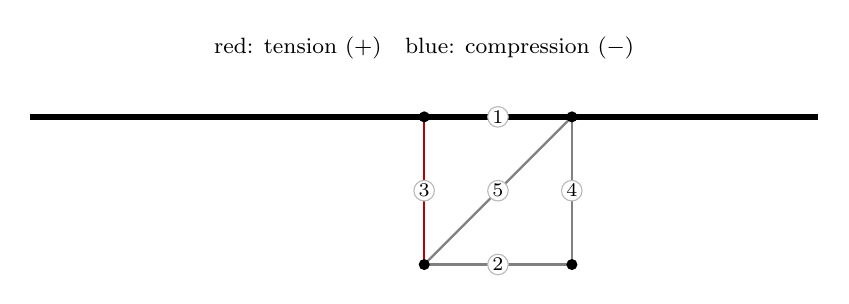
\begin{tikzpicture}[scale=1.250,>=Stealth,line join=round]
  \coordinate (P0) at (0.000,0.000);
  \coordinate (P1) at (4.000,0.000);
  \coordinate (P2) at (8.000,0.000);
  \coordinate (TO1) at (5.500,0.000);
  \coordinate (TU0) at (4.000,-1.500);
  \coordinate (TU1) at (5.500,-1.500);
  \draw[thick,gray] (P1) -- (TO1);
  \draw[thick,gray] (TU0) -- (TU1);
  \draw[thick,red!75!black] (P1) -- (TU0);
  \draw[thick,gray] (TO1) -- (TU1);
  \draw[thick,gray] (TU0) -- (TO1);
  \draw[line width=2pt] (P0) -- (P1);
  \draw[line width=2pt] (P1) -- (P2);
  \fill (P1) circle (1.6pt);
  \fill (TO1) circle (1.6pt);
  \fill (TU0) circle (1.6pt);
  \fill (TU1) circle (1.6pt);
  \node[circle,fill=white,draw=gray!55,inner sep=0.5pt,font=\scriptsize] at (4.750,0.000) {1};
  \node[circle,fill=white,draw=gray!55,inner sep=0.5pt,font=\scriptsize] at (4.750,-1.500) {2};
  \node[circle,fill=white,draw=gray!55,inner sep=0.5pt,font=\scriptsize] at (4.000,-0.750) {3};
  \node[circle,fill=white,draw=gray!55,inner sep=0.5pt,font=\scriptsize] at (5.500,-0.750) {4};
  \node[circle,fill=white,draw=gray!55,inner sep=0.5pt,font=\scriptsize] at (4.750,-0.750) {5};
  \node[font=\footnotesize] at (4.00,0.70) {red: tension $(+)$\quad blue: compression $(-)$};
\end{tikzpicture}
\end{center}
\par\medskip\textbf{4.\ Section-force diagrams of the beams}\par
\begin{center}
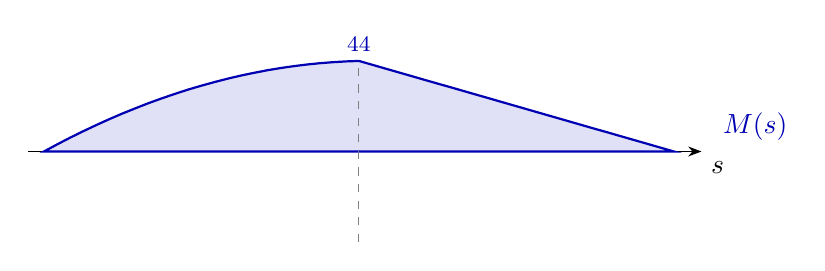
\begin{tikzpicture}[>=Stealth]
  \draw[->] (-0.2,0) -- (8.35,0) node[below right]{$s$};
  \filldraw[fill=blue!70!black!12,draw=blue!70!black,thick] (0,0) -- plot coordinates {(0.000,0.000) (0.167,0.090) (0.333,0.176) (0.500,0.258) (0.667,0.337) (0.833,0.412) (1.000,0.484) (1.167,0.551) (1.333,0.616) (1.500,0.676) (1.667,0.733) (1.833,0.787) (2.000,0.836) (2.167,0.882) (2.333,0.925) (2.500,0.964) (2.667,0.999) (2.833,1.031) (3.000,1.059) (3.167,1.083) (3.333,1.104) (3.500,1.121) (3.667,1.134) (3.833,1.144) (4.000,1.150) (4.000,1.150) (4.167,1.102) (4.333,1.054) (4.500,1.006) (4.667,0.958) (4.833,0.910) (5.000,0.862) (5.167,0.815) (5.333,0.767) (5.500,0.719) (5.667,0.671) (5.833,0.623) (6.000,0.575) (6.167,0.527) (6.333,0.479) (6.500,0.431) (6.667,0.383) (6.833,0.335) (7.000,0.287) (7.167,0.240) (7.333,0.192) (7.500,0.144) (7.667,0.096) (7.833,0.048) (8.000,0.000)} -- (8.000,0) -- cycle;
  \draw[gray,dashed,thin] (4.000,-1.15) -- (4.000,1.15);
  \node[above,blue!70!black,font=\footnotesize] at (4.000,1.150) {44};
  \node[blue!70!black,right] at (8.50,0.32) {$M(s)$};
\end{tikzpicture}\\[5pt]
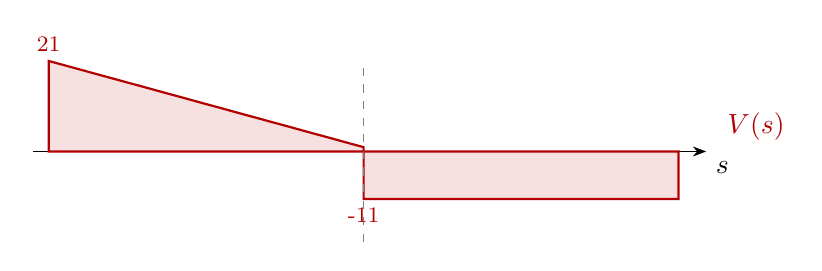
\begin{tikzpicture}[>=Stealth]
  \draw[->] (-0.2,0) -- (8.35,0) node[below right]{$s$};
  \filldraw[fill=red!70!black!12,draw=red!70!black,thick] (0,0) -- plot coordinates {(0.000,1.150) (0.167,1.104) (0.333,1.059) (0.500,1.013) (0.667,0.967) (0.833,0.922) (1.000,0.876) (1.167,0.831) (1.333,0.785) (1.500,0.739) (1.667,0.694) (1.833,0.648) (2.000,0.602) (2.167,0.557) (2.333,0.511) (2.500,0.465) (2.667,0.420) (2.833,0.374) (3.000,0.329) (3.167,0.283) (3.333,0.237) (3.500,0.192) (3.667,0.146) (3.833,0.100) (4.000,0.055) (4.000,-0.602) (4.167,-0.602) (4.333,-0.602) (4.500,-0.602) (4.667,-0.602) (4.833,-0.602) (5.000,-0.602) (5.167,-0.602) (5.333,-0.602) (5.500,-0.602) (5.667,-0.602) (5.833,-0.602) (6.000,-0.602) (6.167,-0.602) (6.333,-0.602) (6.500,-0.602) (6.667,-0.602) (6.833,-0.602) (7.000,-0.602) (7.167,-0.602) (7.333,-0.602) (7.500,-0.602) (7.667,-0.602) (7.833,-0.602) (8.000,-0.602)} -- (8.000,0) -- cycle;
  \draw[gray,dashed,thin] (4.000,-1.15) -- (4.000,1.15);
  \node[above,red!70!black,font=\footnotesize] at (0.000,1.150) {21};
  \node[below,red!70!black,font=\footnotesize] at (4.000,-0.602) {-11};
  \node[red!70!black,right] at (8.50,0.32) {$V(s)$};
\end{tikzpicture}\\[5pt]
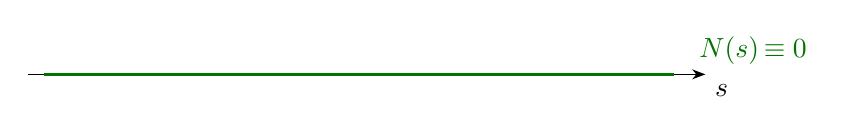
\begin{tikzpicture}[>=Stealth]
  \draw[->] (-0.2,0) -- (8.40,0) node[below right]{$s$};
  \draw[green!45!black,very thick] (0,0) -- (8,0);
  \node[green!45!black,right] at (8.2,0.3) {$N(s)$\,$\equiv 0$};
\end{tikzpicture}\\[10pt]
\end{center}
\end{document}